\section{Thực hiện mạch đọc ADC}

\subsection{Lưu đồ giải thuật của mạch đọc ADC}

Sử dụng ATmega328P để thực hiện xử lý dữ liệu gửi từ ADS1115 về thông qua các chân như sau:

\begin{figure}[H]
	\centering
	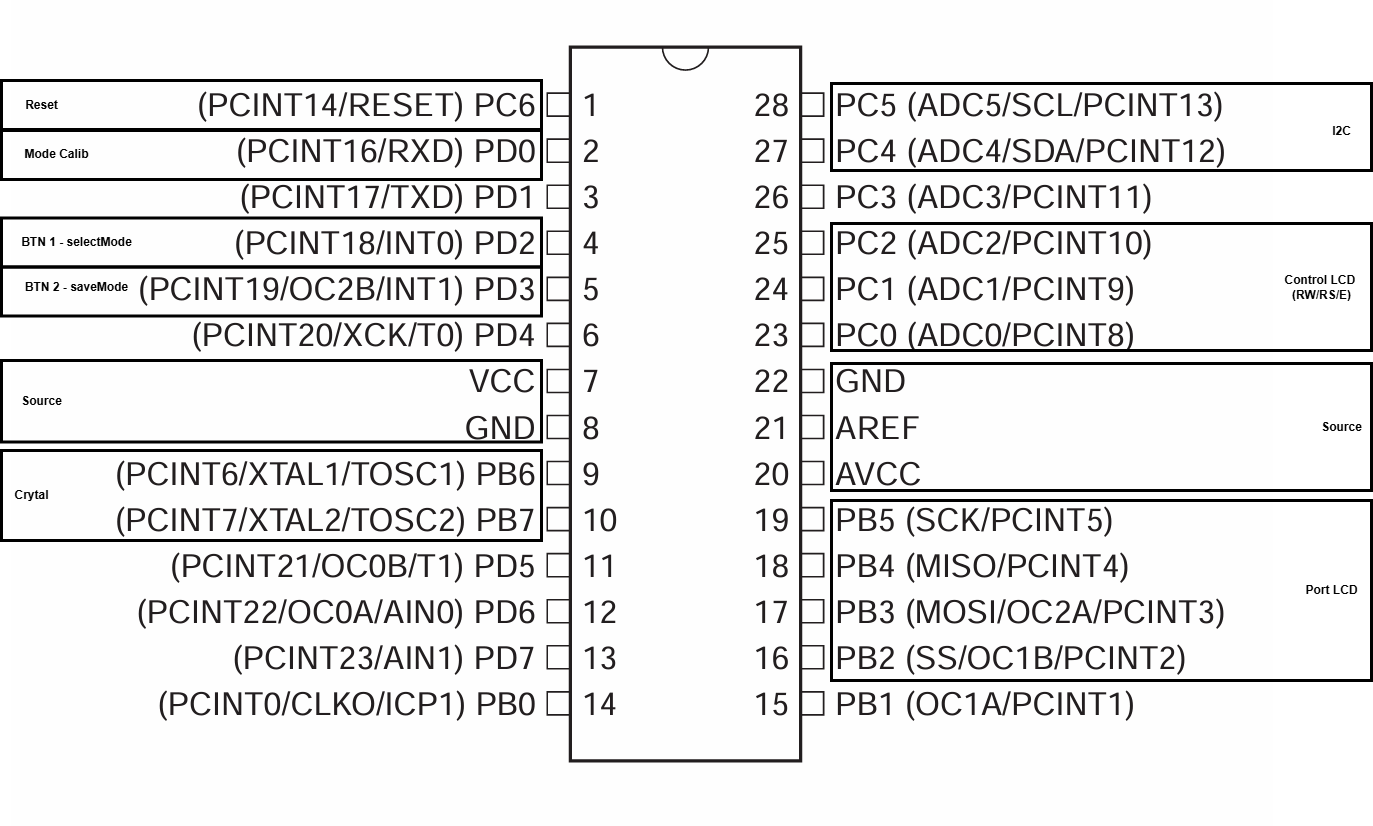
\includegraphics[width=.8\linewidth]{./my-chapters/my-images/PCB_ADC/ADC_spec_mapping.png}
	\caption{Sơ đồ kết nối chân trên ATmega328P.}
\end{figure}

\begin{figure}[H]
	\centering
	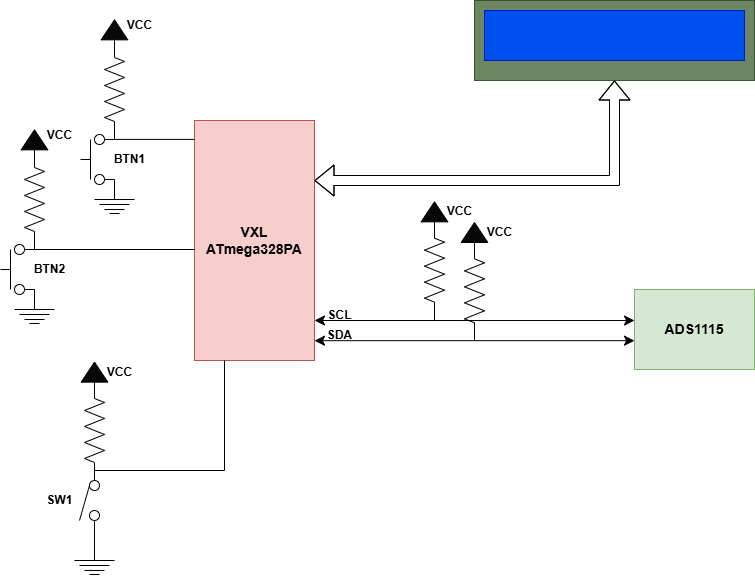
\includegraphics[width=.8\linewidth]{./my-chapters/my-images/PCB_ADC/ADC_spec_overview_connect.png}
	\caption{Sơ đồ kết nối tổng quan cho mạch đọc ADC.}
\end{figure}

\begin{figure}[H]
	\centering
	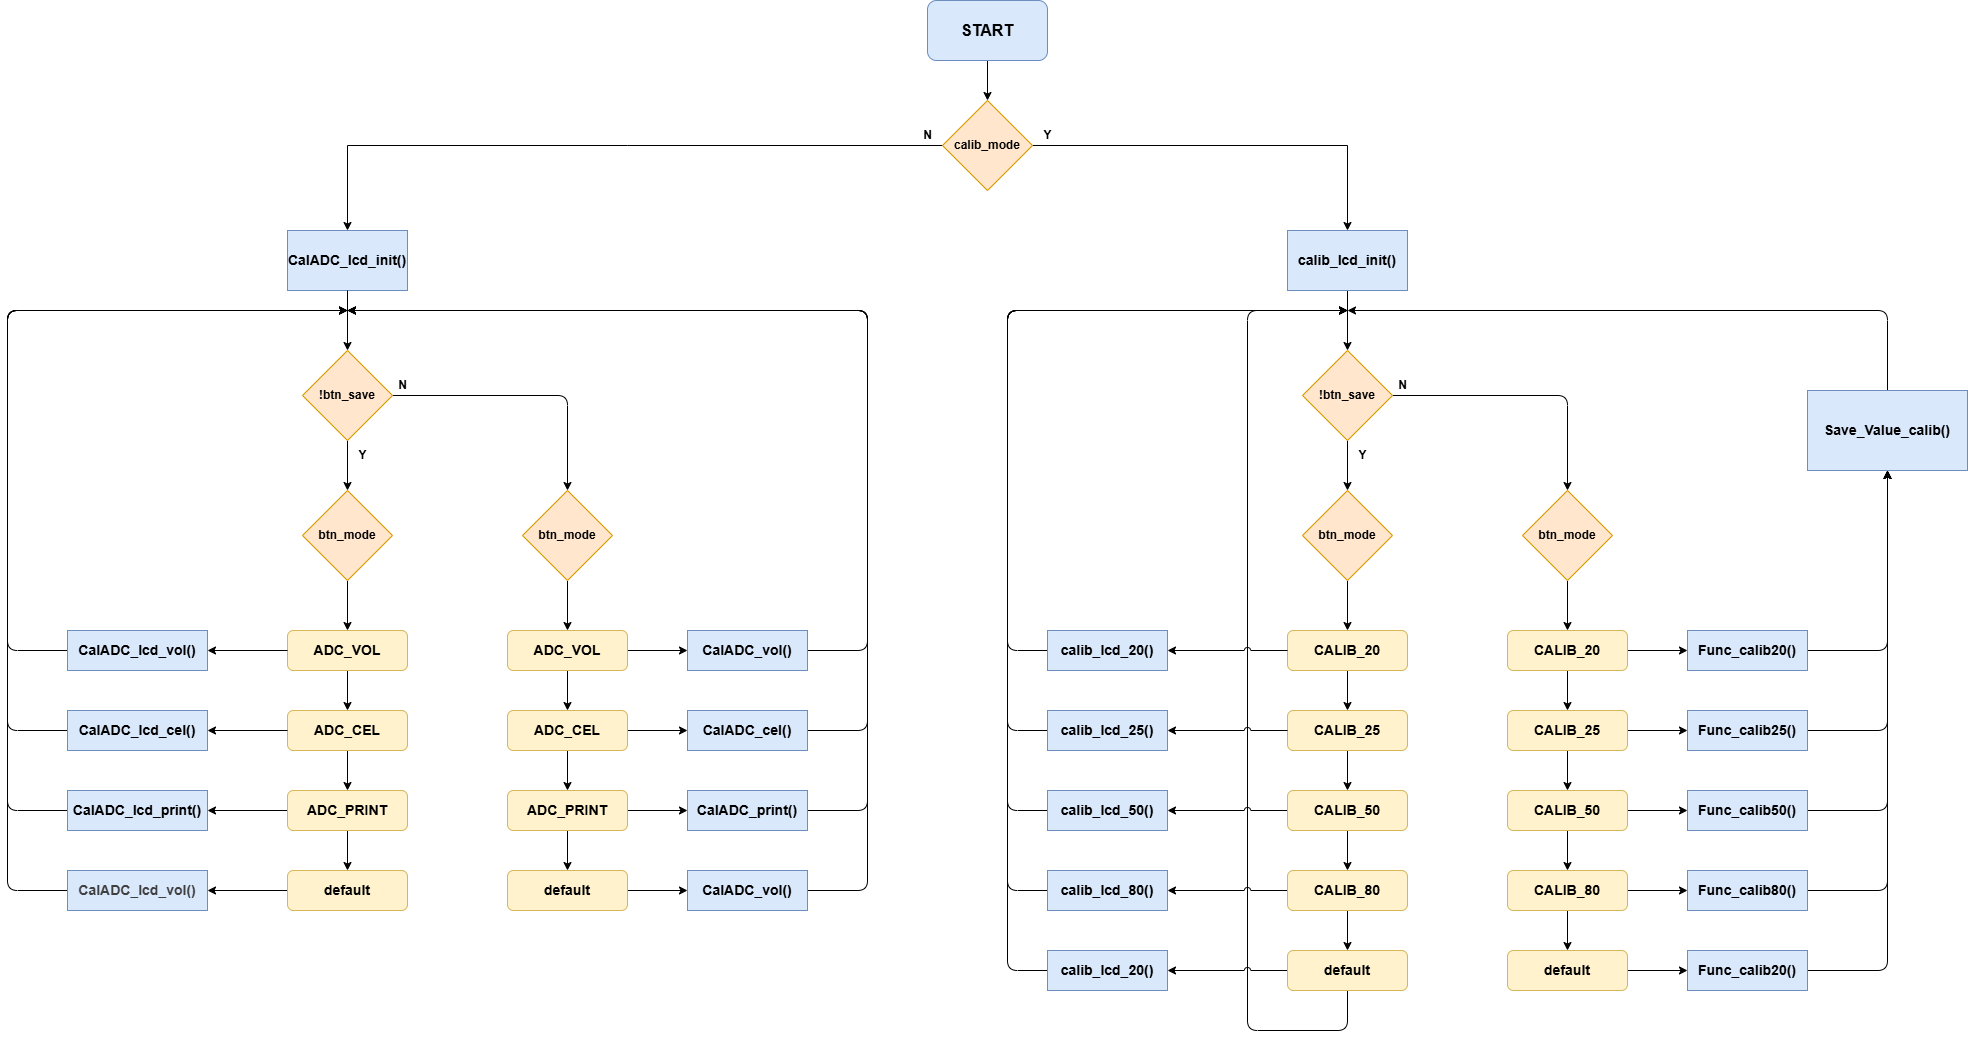
\includegraphics[width=.8\linewidth]{./my-chapters/my-images/PCB_ADC/overflow_diagram.png}
	\caption{Flowchart của mạch đo mạch ADC.}
\end{figure}

\subsection{Mạch đọc ADC}

\begin{figure}[H]
	\centering
	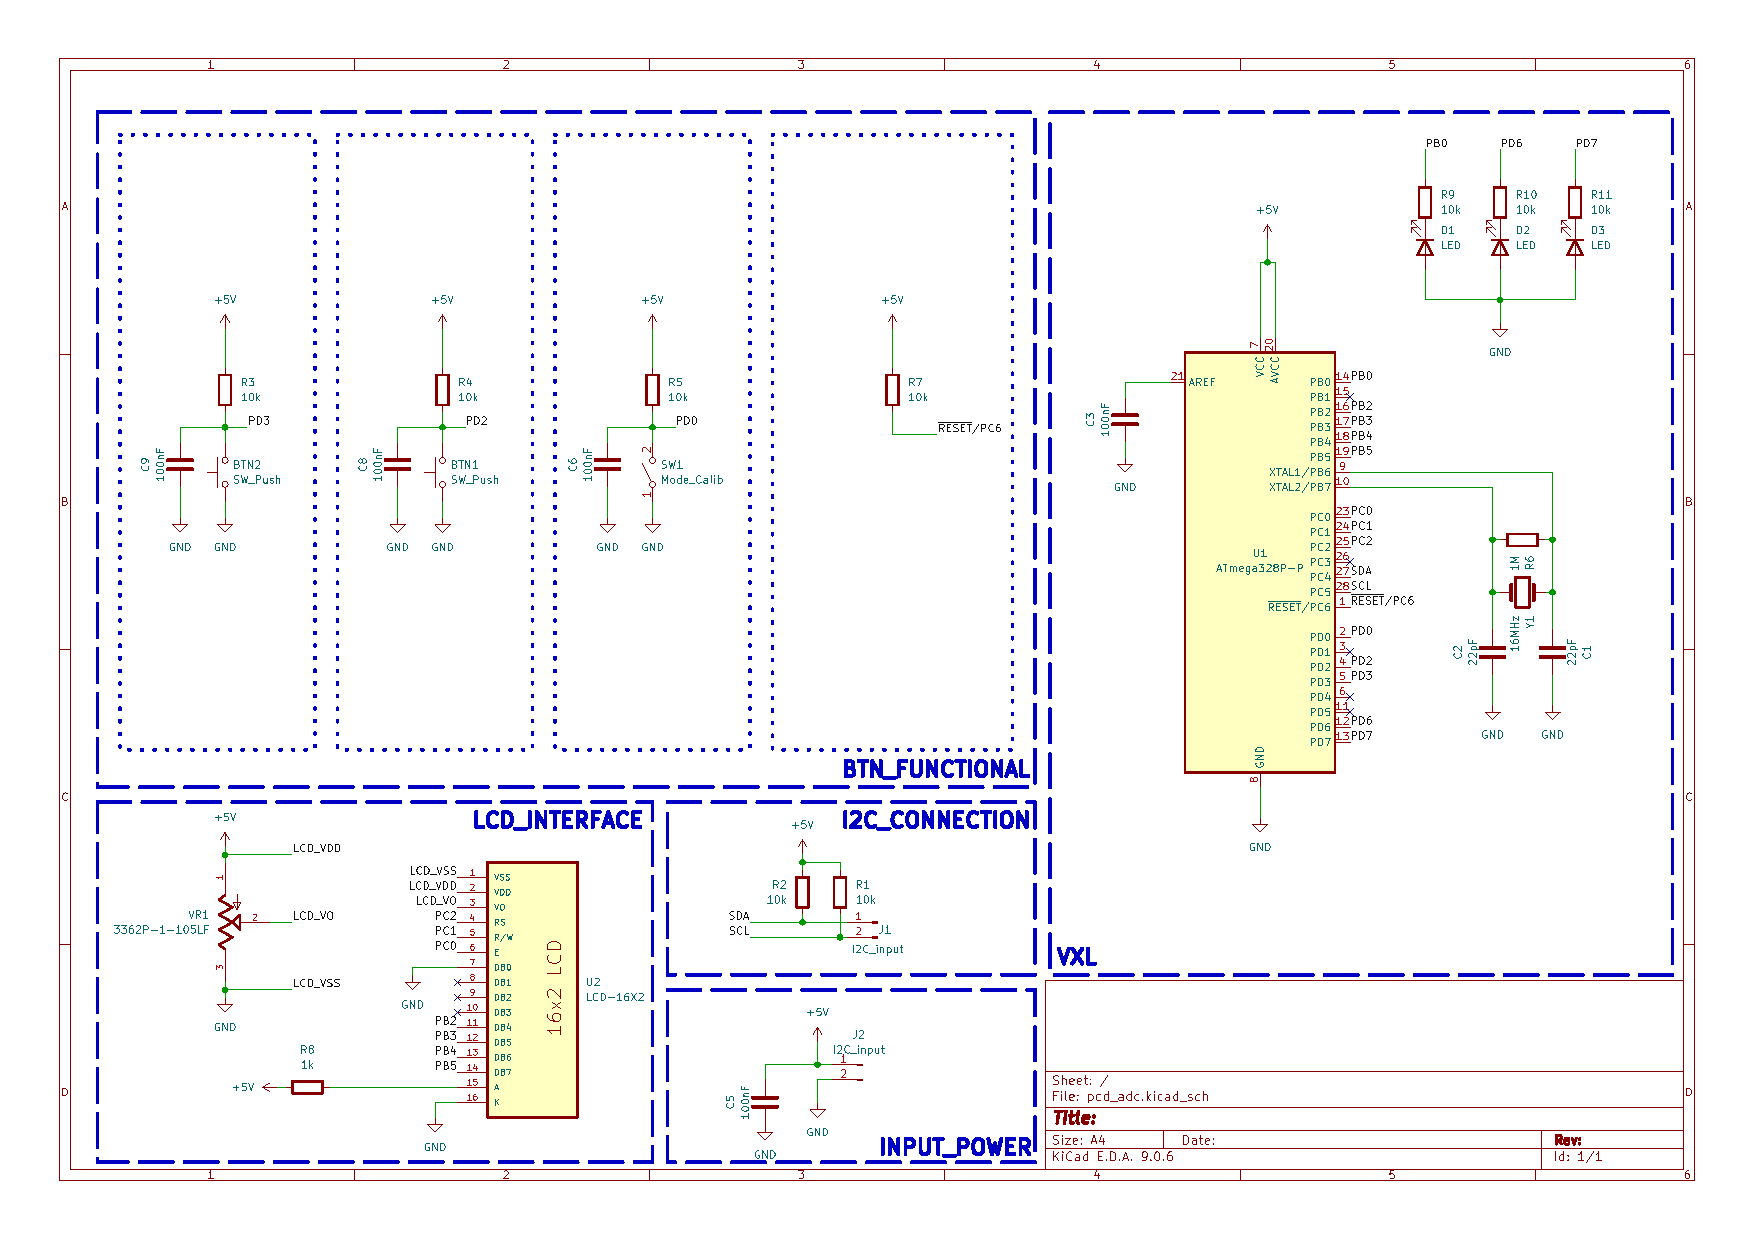
\includegraphics[width=\linewidth]{./my-chapters/my-diagrams/pcd_adc.pdf}
	\caption{Schematic của mạch đọc ADC.}
\end{figure}

\begin{figure}[H]
	\centering
	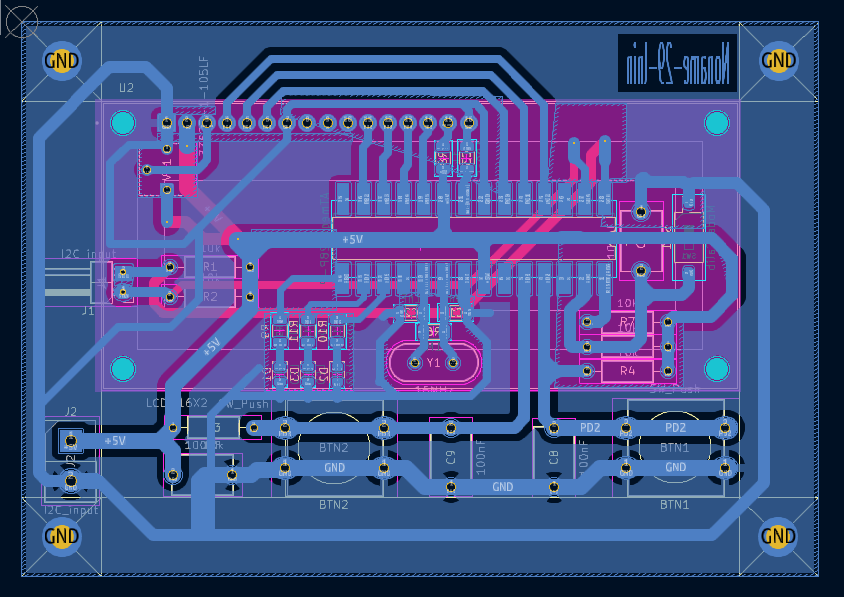
\includegraphics[width=.8\linewidth]{my-chapters/my-images/PCB_ADC/pcb_adc.png}
	\caption{Layout của mạch đọc ADC.}
\end{figure}

\begin{figure}[H]
	\centering
	\begin{minipage}{.45\linewidth}
		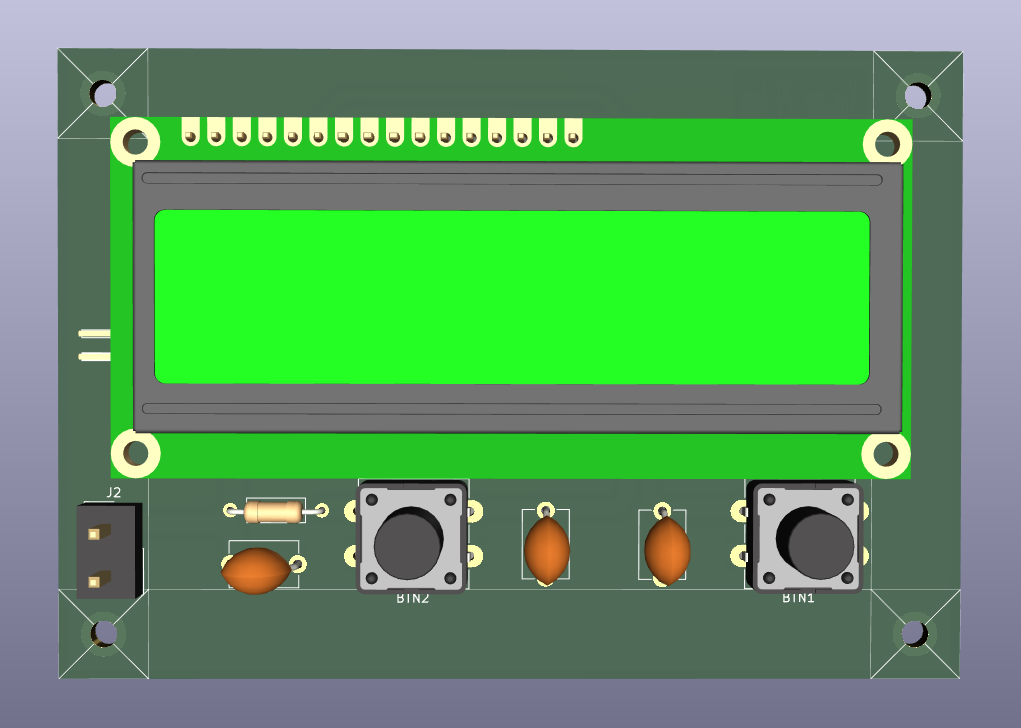
\includegraphics[width=\linewidth]{my-chapters/my-images/PCB_ADC/3D_topview.png}
	\end{minipage}
	\begin{minipage}{.45\linewidth}
		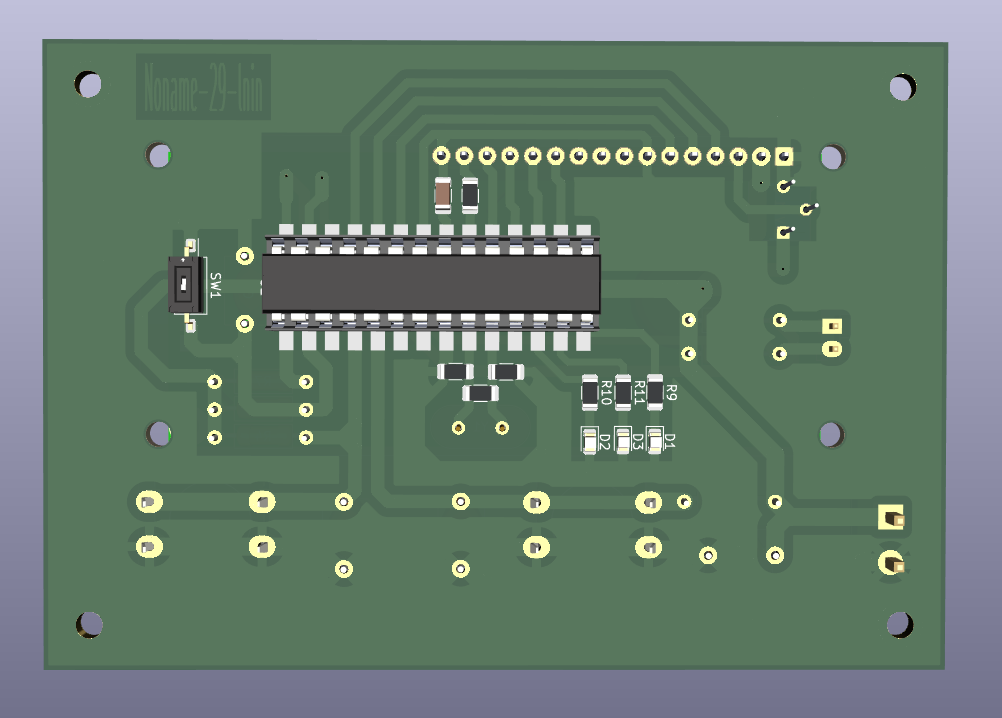
\includegraphics[width=\linewidth]{my-chapters/my-images/PCB_ADC/3D_underview.png}
	\end{minipage}
	\caption{3D của mạch đọc ADC.}
\end{figure}

\begin{figure}[H]
	\centering
	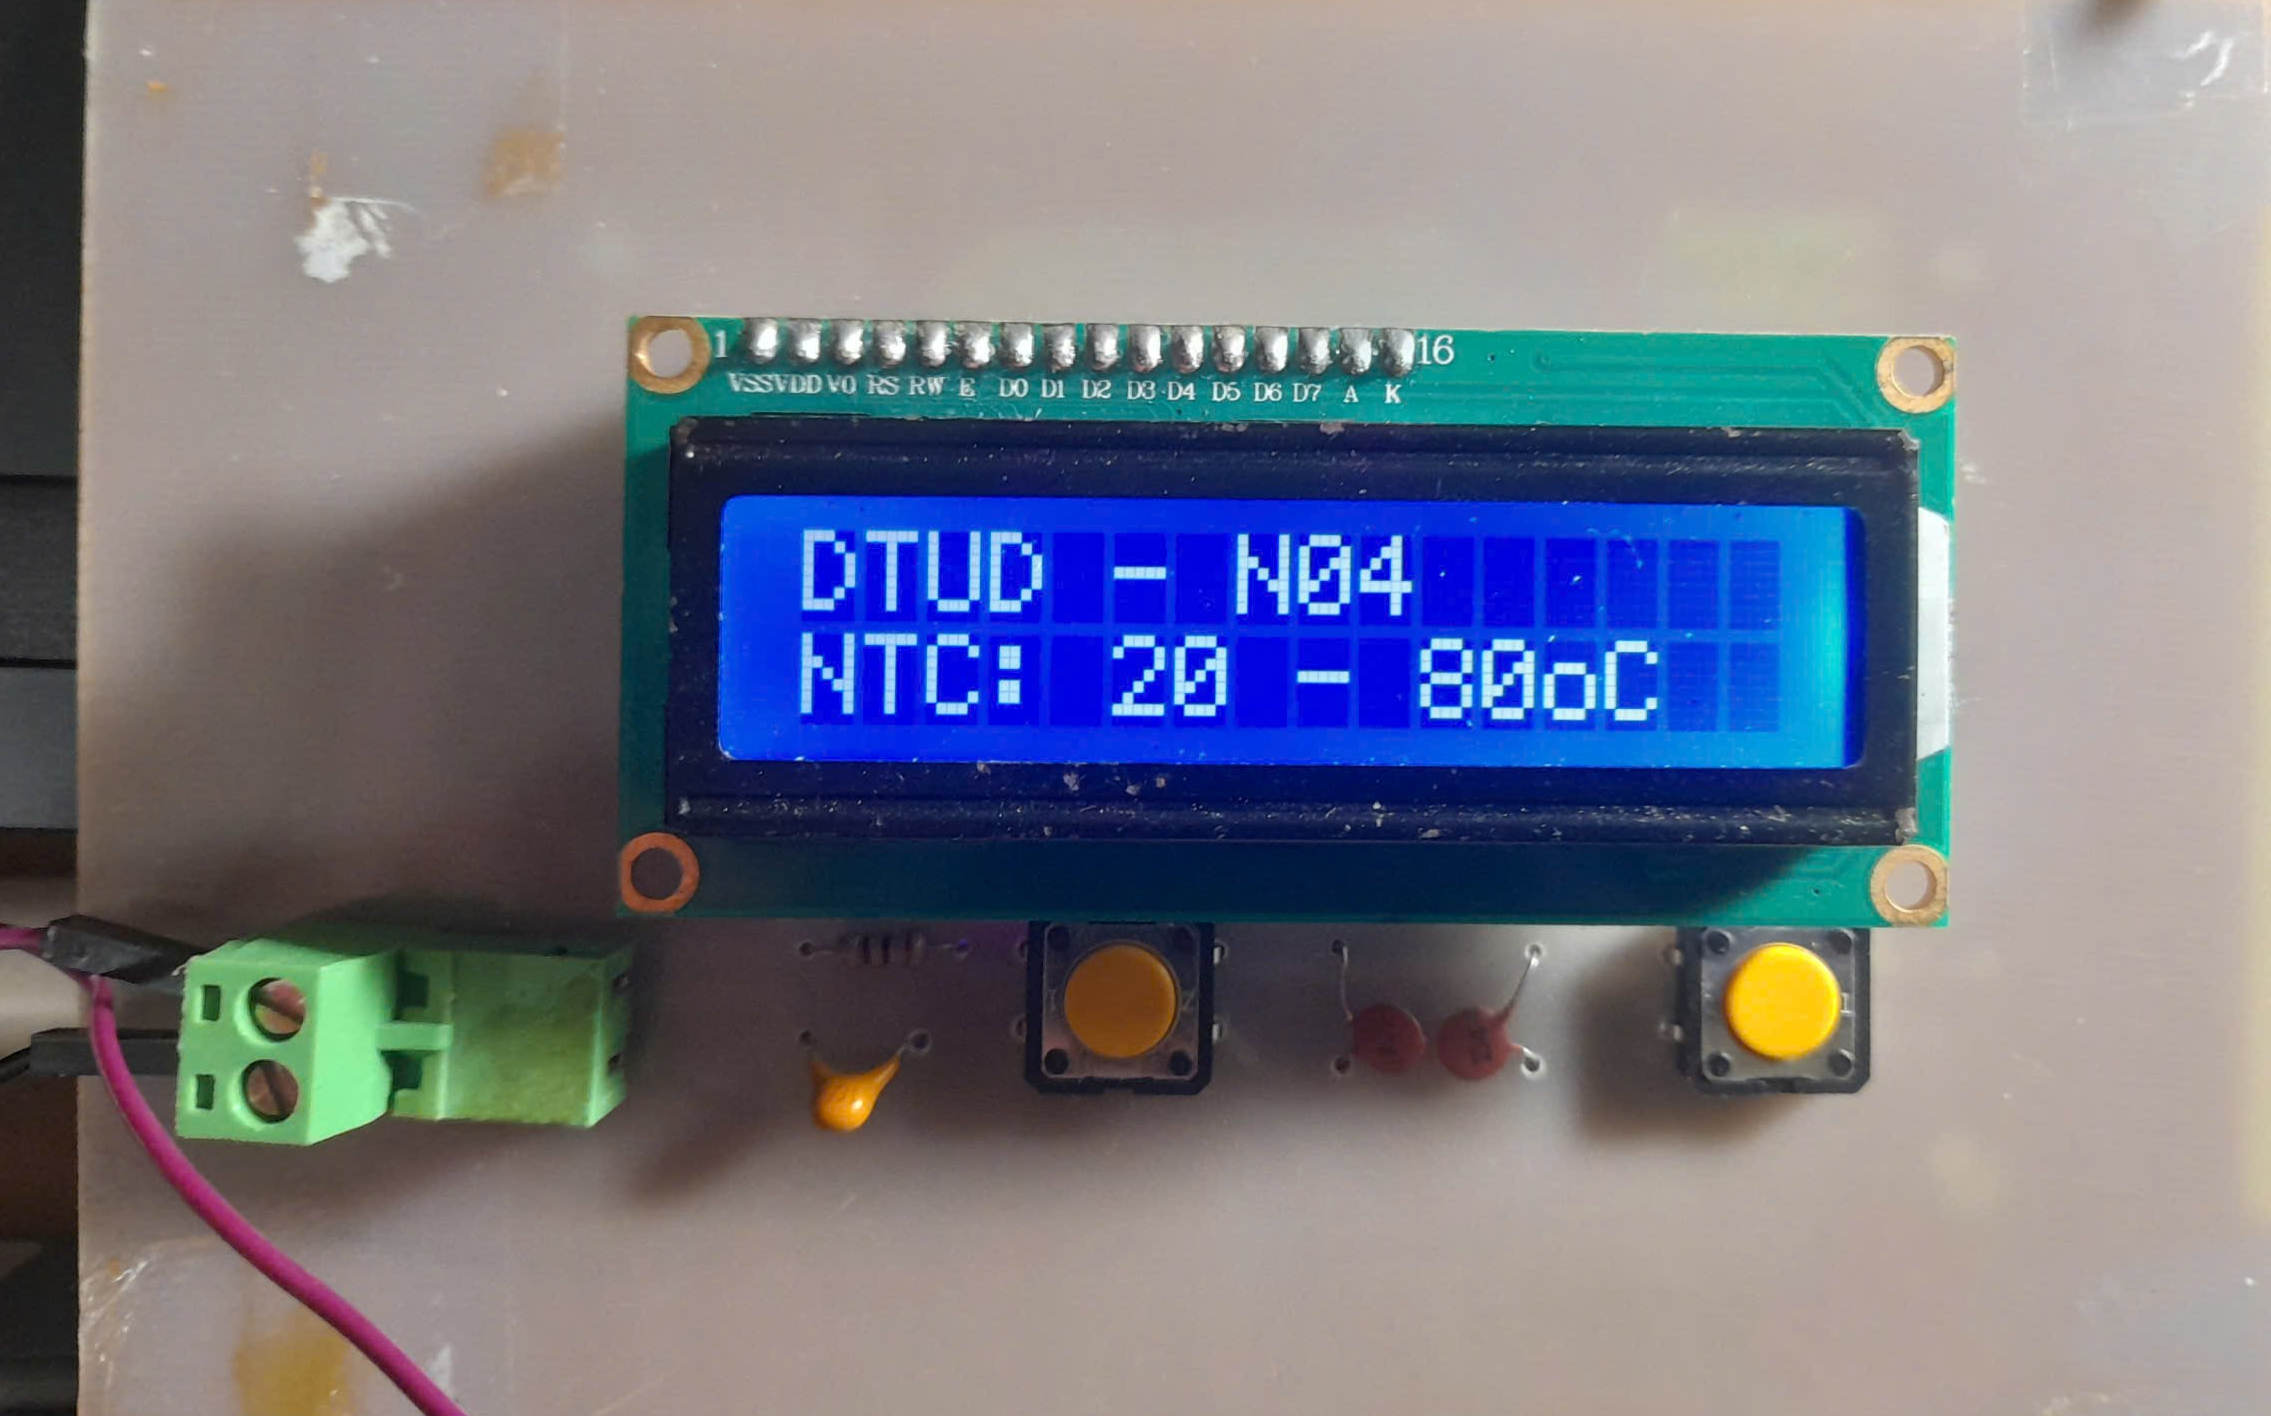
\includegraphics[width=.8\linewidth]{my-chapters/my-images/PCB_ADC/Real_ADCPCB.png}
	\caption{Mạch thực tế của mạch ADC.}
\end{figure}